\chapter{Design and implementation}
\label{chapter:DesignAndImplementation}
\section{Overview}
\label{section:Overview}

To approach the objectives of this project, we've focused on building a complete infrastructure based on microservices ready to be deployed on the cloud. In the course of this chapter, we will explain how we developed and configured several components, each one serving a  different task of our system.

Docker will help us to containerize each component and make it system-independent, and Kubernetes will help us orchestrate all the components and manage their scale and status. We will dedicate a subsection on each component to explain how we containerized and deployed it to the cluster. 

Inside Kubernetes, we will deploy these components:

\begin{itemize}
\item A web application where the users will be able to make predictions and interact with our system.
\item A MongoDB database to store all the raw and processed data.
\item Several FIWARE components that will enable the communication between our services, and manage the information context.
\item A Spark Cluster, that will run our machine learning model and process the data.
\item Other components to automate some tasks.
\end{itemize}

\begin{figure}[H]
	\centering
	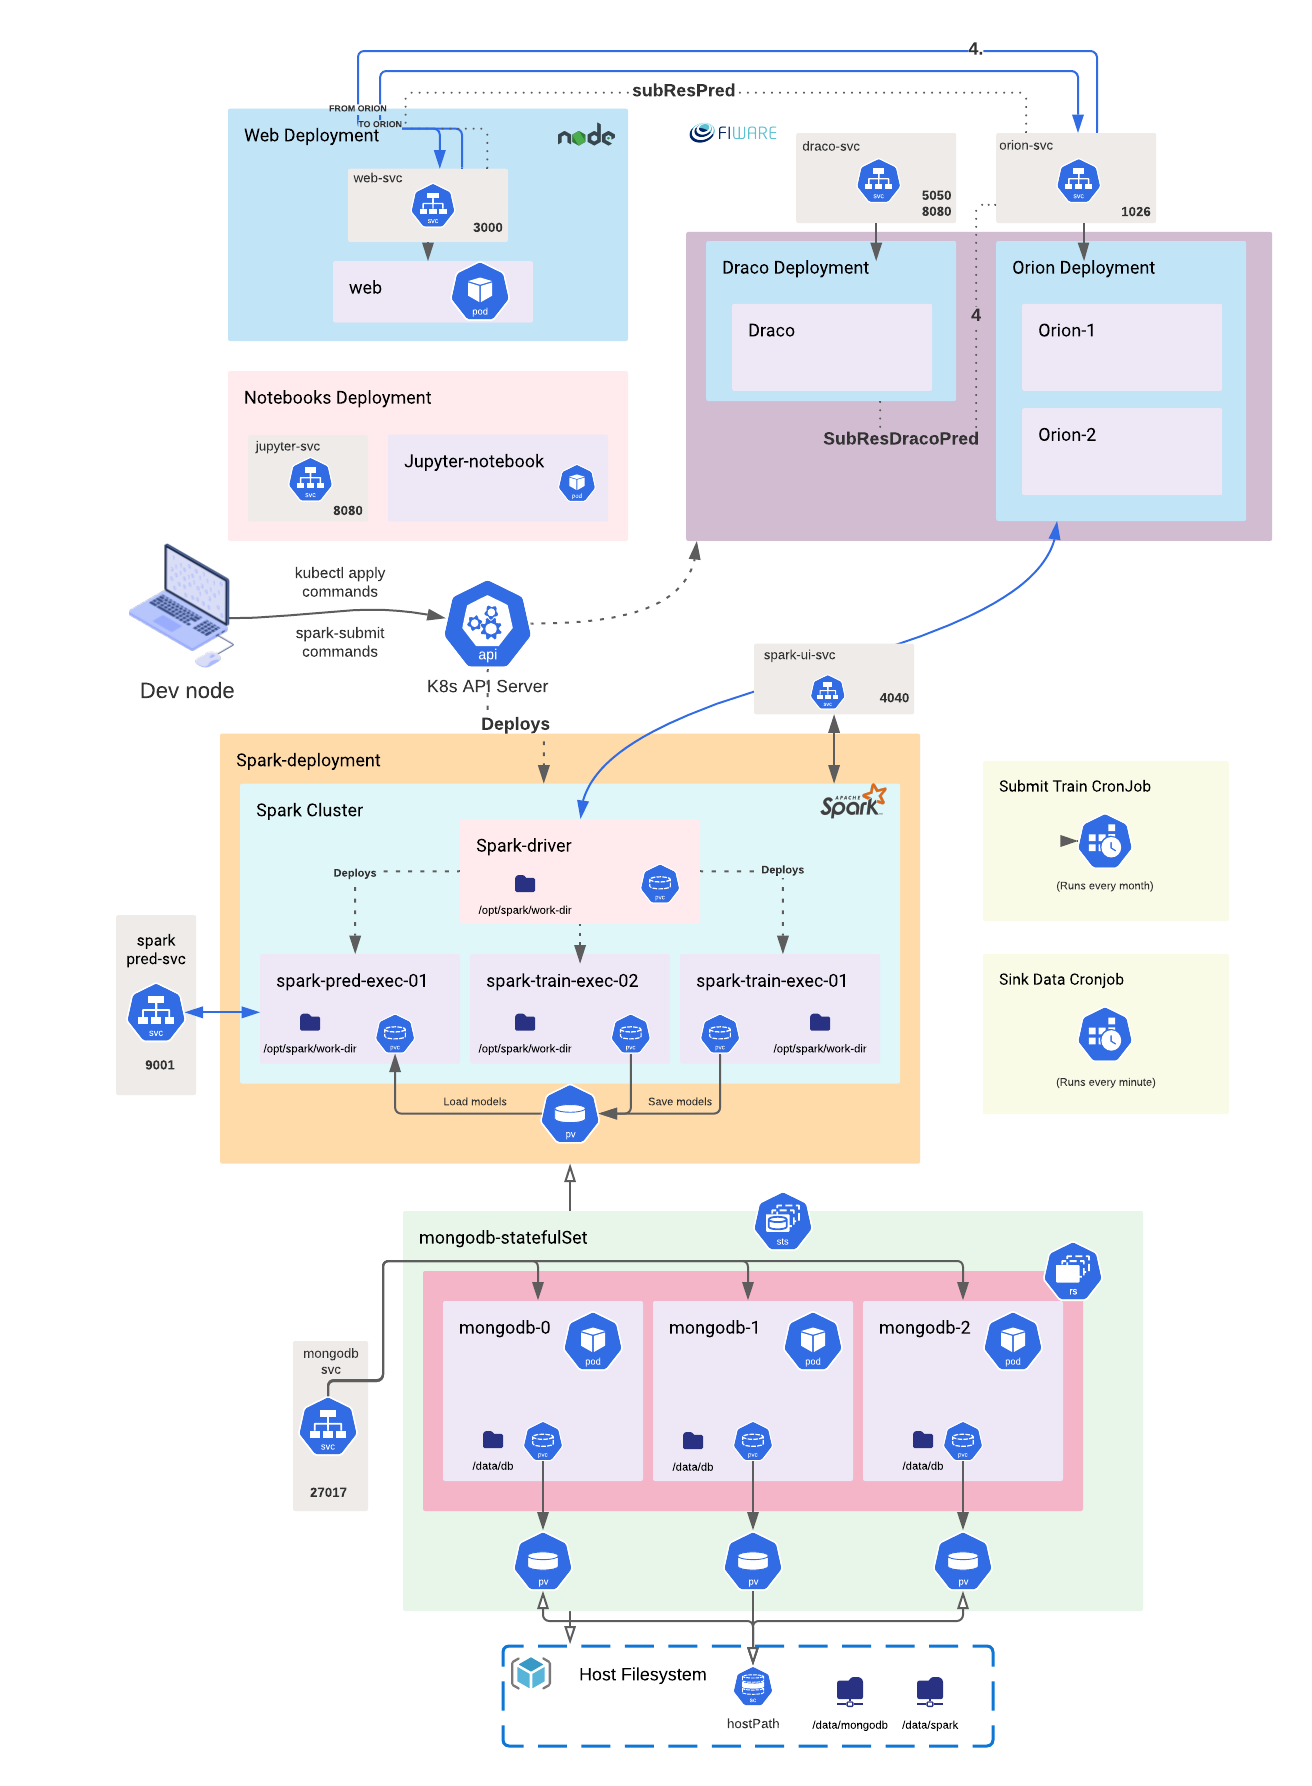
\includegraphics[width=1\linewidth]{imagenes/diagram.png}
	\caption{Representation of the Kubernetes architecture of the whole deployment.}
	\label{diagram}
\end{figure}

As cloud services providers like AWS or Google Cloud do not have free plans for a project with the resource requirements that Spark and Machine Learning add to our development,  we decided to use Minikube to host our Kubernetes cluster. Minikube is a single-node Kubernetes deployment focused on helping developers and administrators to set up a simple Kubernetes cluster in their local machine. Additionally, we will set up a docker registry in Docker Hub to store our images. 

Before going deeper into the development of the system, I would like to point out that all the code for this project is hosted in a Github Repository, and to replicate the cluster in another environment there is a dedicated script named \textit{create\_cluster.sh} that will do all the work. (\ref{CreateCluster})

\textit{Github repository}: https://github.com/tonihurtado/fiware-kube-ml-parking

\section{Web Application}
\label{section:WebApp}

The web application will be the interface for the users of the system, and it can also be seen as the starting point of the data flow.

\begin{figure}[H]
	\centering
	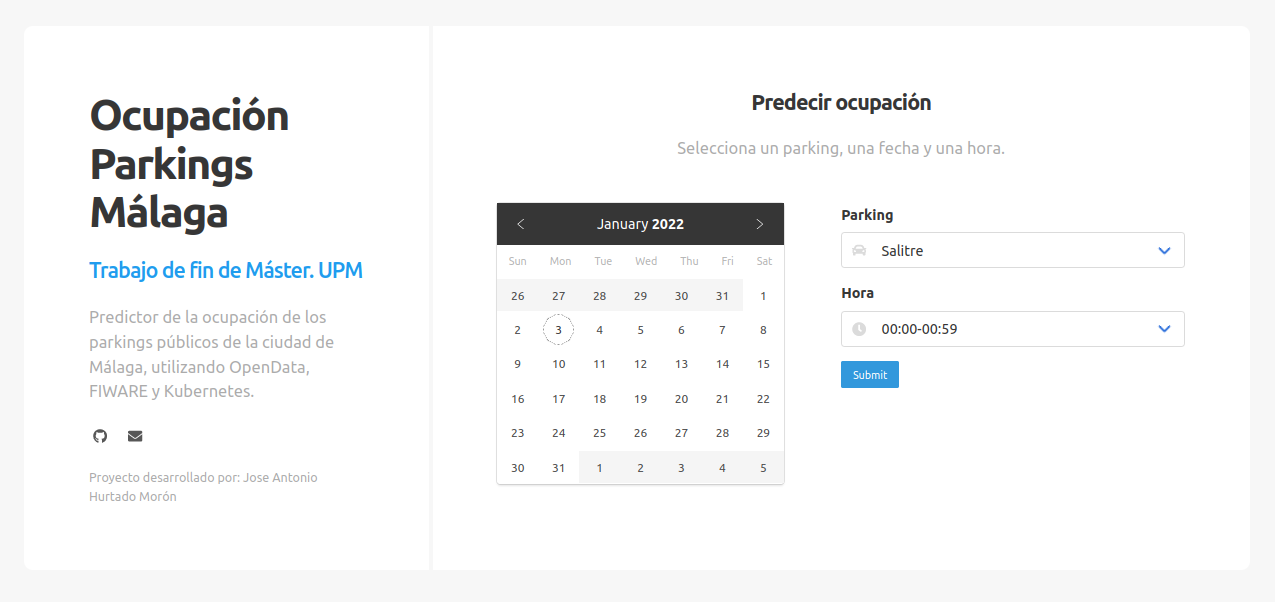
\includegraphics[width=1\linewidth]{imagenes/website.png}
	\caption{User Interface of the web application.}
	\label{website}
\end{figure}

The layout is simple, with a section on the left where the project is briefly described, and a form on the right where the user can select the inputs. Clicking on the button placed in the upper right corner, we can also access a list showing the previous prediction requests, ordered descending according to the date.

\subsection{Architecture}
\label{section:WebAppArchitecture}

The \textbf{frontend} has been developed with HTML, and the design is pure CSS but generated using the Bulma framework, which provides ready-to-use frontend components that you can easily combine.

The \textbf{backend} of this web app has been developed in Javascript, using the NodeJS framework. Express will serve as a tool to design the API, and Mongoose as the client to connect to the database. The whole backend code will be defined in only one file, \textit{app.js.} The express API will define three endpoints: 

\begin{itemize}
\item GET \textit{/ →} Serves the frontend files.
\item GET \textit{/predictions →} Return the list of past predictions fetched from the database.
\item POST \textit{/notify →}  Listens to the prediction notification from Orion.
\end{itemize}

For the \textbf{communication} between both components, we are using Socket.io, as the application will have to wait for the whole flow (context broker queue, Spark Stream processing for prediction with the model and the trip back) before printing the prediction in the layout again and writing the result to the database. The frontend will open the socket on the form submission and will send a PREDICT message with the data. The possible messages over the socket are:


\begin{itemize}
    \item PREDICT: Start a prediction request with the data provided in the payload.
    \item CONFIRMATION: The Orion Broker has received the data and sent it to Spark for its procession. Triggers load spinner on the UI.
    \item ERROR: Communication with Orion Failed. Displays an error message on the UI.
    \item PREDICTION: The prediction succeeded and has been received. It will render the predicted value on the UI.
\end{itemize}

\begin{figure}[H]
	\centering
	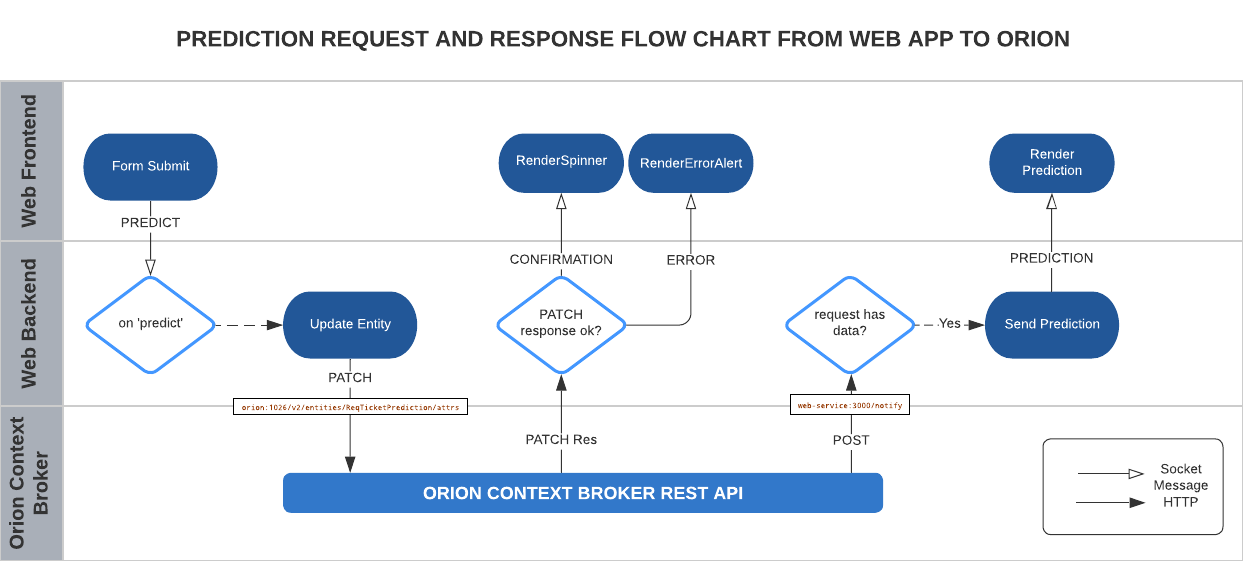
\includegraphics[width=0.9\linewidth]{imagenes/flow-chart-web-orion.png}
	\caption{Prediction request and response flow chart from webapp to orion.}
	\label{flow-chart-web-orion}
\end{figure}

\subsection{Containerization and deployment in Kubernetes}

To deploy our application to the cluster, we should first create a docker container to wrap it. Our docker image will be built based on the node official image, version 12.18.1. We will also pass some environment variables to the image, specifying the different endpoints of the Kubernetes context that the app will need. 

We will create a Deployment in Kubernetes for this components. With a deployment, we will guarantee that we have always one replica of our container running, and if it fails for some reason, the kubelet service will make sure that the container is deployed again. Also, we will create a LoadBalancer service to expose the port 3000 to our local machine, making use of the minikube's services tool.

\begin{figure}[H]
	\centering
	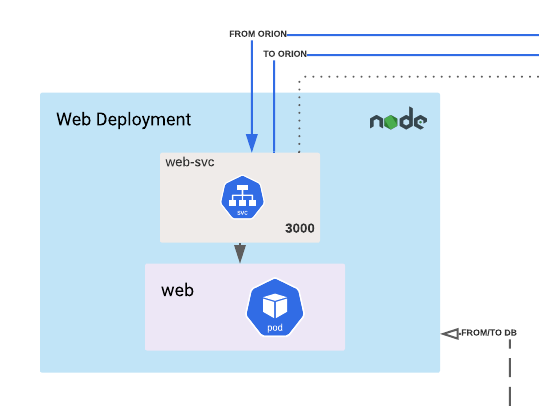
\includegraphics[width=0.5\linewidth]{imagenes/diagram-web-kube.png}
	\caption{Representation of the Kubernetes architecture of the web deployment.}
	\label{diagram-web-kube}
\end{figure}

\clearpage

\section{Database and Data Schemas}
\label{section:DB}

We chose to use MongoDB as our database service for multiple reasons. First and most important, Orion is designed to use MongoDB as the database to store it's context, so we needed it for this purpose. Also, most of the data we are going to work with is already in JSON format, as the NGSI linked data can be serialized to JSON-LD by default. Finally, both Javascript applications and Spark are prepare to easily work with JSON data. So having a central database for all this services was the best option.

As we want our database to be reliable and scalable too, we opted to deploy mongod in replica set mode and as a Kubernetes StatefulSet.

\begin{itemize}
  \item A \textbf{Replica-set} in MongoDB is a cluster of servers that implements replication and automated failover. With this deployment architecture, we will have multiple mongod processes in different Pods managing the same database, and because of this, we will acquire redundancy and a better data availability.
  \item A \textbf{StatefulSet} is the object defined by Kubernetes to manage the deployment of stateful applications, that means, applications with multiple replicas of the same pod that need some guarantees about the order and the state of the running pods. Is the recomended object when deploying databases in cluster mode. (\ref{MongoKubernetes})
\end{itemize}

\begin{figure}[H]
	\centering
	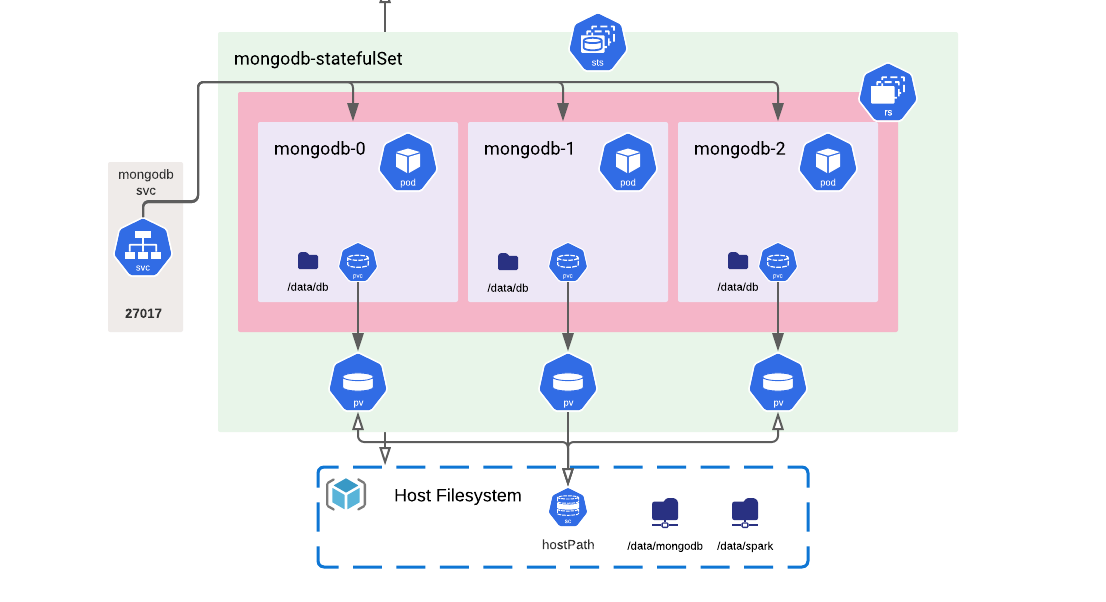
\includegraphics[width=1\linewidth]{imagenes/diagram-db.png}
	\caption{Diagram of the Kubernetes architecture for the database.}
	\label{diagram-db}
\end{figure}

We will also create a PersistentVolume resource, using our hostPath directory as mount point. This will allow us to save the data in a directory of the host where Minikube is running, so we won't loose the data when the cluster goes down. A PersistentVolumeClaim is also needed to map this PersistentVolume with each of the Pods running the mongod process.

Our respective services using the replicaset will automatically create three different databases:

\begin{itemize}
  \item \textbf{Orion}: Created by orion to store information relative to it's entities, subscriptions and internal configuration.
  \item \textbf{Tfm}: We will use this database to save the raw data gathered from the Open Data Platform. This data will be used later to train our model. Another collections with testing purposes will be also created here.
  \item \textbf{Sth\_test}: This database will be created by Draco, to save the list of past predictions requested by the web application. 
\end{itemize}

\clearpage

\section{Fiware: Orion and Draco}
\label{section:Fiware}

The FIWARE components will act as the backbone of our system, providing us with tools to manage our information context and communicate the different services.

The \textbf{Orion Context Broker} will be the main component of our deployment and will administer the context information and data in a decentralized and scalable manner. Orion implements the  FIWARE NGSIv2 API to manage the context information. With this restful API  NGSI, we will be able to perform updates, queries, and change subscriptions on our entities, and also asynchronously connect most of our microservices.

On the other side, we will also use \textbf{Draco}, a FIWARE tool based on Apache NIFI that will power up some of our dataflows. Draco will allow us to create a data pipeline from Orion to our database, so the predictions that go through the Context Broker will be processed and stored in an asynchronous way, so the webapp is able to request them in the future.


\subsection{Orion entities}

In Orion, entities describe the data structure of an object that could be processed by the broker, using the NGSIv2 specification. For example, the temperature of a room could be an entity. 

For our requirements in this project, we only need two different entities. These entities will describe to Orion the kind of objects that can be sent to the broker and their structure. For each attribute of the entity, we will define a name, a value, and a type, which are already defined in the NGSIv2 specification and will help us standardize our data with other context producers and consumers. In this case, we have these two entities:

\textbf{ReqTicketPrediction}:

Defines the input data for our prediction request data flow. The values are set to 0 by default, as we will update this entity with new information every time a user performs a new prediction on the webapp. (\ref{ReqTicketPrediction})

\textbf{ResTicketPrediction}:

Defines the output data for our prediction request data flow. This entity will be updated by the Spark Streaming app, every time a new value is predicted for an input request. (\ref{ResTicketPrediction})


\subsection{Orion subscriptions}

Subscriptions are the mechanism used by Orion to generate a reactive response based on changes in the context information defined by the entities. In our case, we will need to define subscriptions for the predictions requests and responses, and we will also define an additional subscription for Draco.

In Orion, subscriptions are linked to an entity and triggered under the change of certain conditions (i.e. an update of an attribute). Once a subscription is triggered, it will send the specified attributes over the specified notification channel. In our project, this will be an HTTP POST request to the URL of another component of our system. This way, we can asynchronously communicate the components in our data flow using FIWARE standards and controlling the triggering parameters. The defined subscriptions are:

\textbf{subscribeReqPredictionTicket}:

Defines the input data for our prediction request data flow. The values are set to 0 by default, as we will update this entity with new information every time a user performs a new prediction on the webapp. (\ref{subscribeReqPredictionTicket})

\textbf{subscribeResPredictionTicket}:

Defines the output data for our prediction request data flow. This entity will be updated by the Spark Streaming app, every time a new value is predicted for an input request. (\ref{subscribeResPredictionTicket})

\textbf{subscribeResDracoPredictionTicket}:

Defines the subscription that will trigger Draco for post-processing of our prediction. (\ref{subscribeResDracoPredictionTicket})


\subsection{Containerization and deployment in Kubernetes.}

FIWARE provides official and frequently updated docker images for most of their components, and as our project doesn't require any additional configuration to the standart Orion and Draco tools, we will stick to them instead of building our own.

Focusing on Kubernetes configuration, we will define a Deployment to maintain and scale on demand the Orion Pod. As arguments for the configuration of the Orion container, we will specify the database URI and the replica set information, with some additional parameters for improving the performance. The port used for the container will be the default for Orion, 1026. (\ref{OrionKubernetes})

Regarding the Service, we will configure a NodePort service using port 1026 as container port and port 30329 as the external port, as we will need to make HTTP requests from outside of the cluster to configure the entities and subscriptions. (\ref{OrionKubernetesService})

For Draco, Kubernetes configuration will be similar. We will also define a Deployment, with no previous configuration, and, in this case, a normal service exposing both data (5050) and UI (8080) ports. We will use the label service:draco for the match between both components. (\ref{DracoKubernetes} and \ref{DracoKubernetesService})

\subsection{Data flow on Fiware components}

Once we have our components deployed in the cluster, the first step is to configure the Orion entities and subscriptions (just on a fresh start of the containers). We will do that through the NGSIv2 API, doing POST requests from our shell to the configured NodePorts.

To automate this process, we have created a shell script that has all the data already pre-configured. As we are working with Minikube for this example, we only have one node, and we can obtain its IP address by using the *minikube ip* command. Then, we will sequentially call the different scripts. These scripts perform a curl POST command including the object's description in an NGSIv2-compatible JSON format as payload (the JSON we described in the previous section).

\begin{lstlisting}[language=bash,caption=Script to perform the configuration of Orion entities and Subscriptions]
CLUSTER_IP=$(minikube ip)
sh createPredictionEntities.sh $CLUSTER_IP:30329
sh subscribeReqPredictionTicket.sh $CLUSTER_IP:30329
sh subscribeResPredictionTicket.sh $CLUSTER_IP:30329
sh subscribeResDracoPredictionTicket.sh $CLUSTER_IP:30329
\end{lstlisting}

The commands will return a *201 Created* code if everything went ok.

Regarding the database, the configuration is done on the Pod definition template, as we are passing down the parameters to connect to MongoDB. If the connection is successful, Orion will create a new database named Orion, where different collections dedicated to entities, subscriptions, registrations, and internal configurations will be generated.

Once everything is configured, our Context Broker will be ready to interact with other components of our cluster. As we explained, we will update the entities by doing a PATCH request to the API, and if the trigger conditions are met, a notification will be sent to the URL specified in the subscription configuration.

Now, we can improve the flow chart defined in the webapp section by adding Orion to the equation. In the following chart, the interactions between Orion and the surrounding components are explained for the prediction request flow.

\begin{figure}[H]
	\centering
	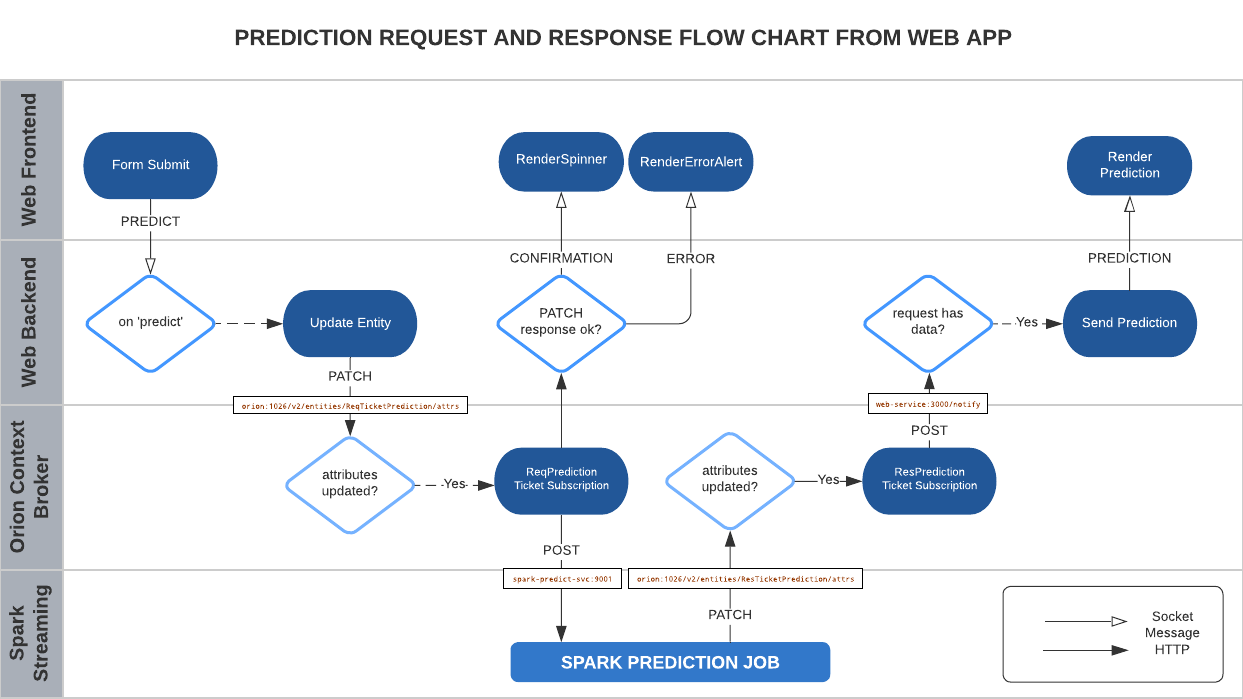
\includegraphics[width=1\linewidth]{imagenes/flow-chart-web-spark.png}
	\caption{Prediction request and response flow chart from webapp to spark.}
	\label{flow-chart-web-spark}
\end{figure}

\subsection{Adding and Configuring Draco}

In the final stages of the development of this proof of concept, we introduced Draco as a tool to help us deal with the processing and storage of the predicted value. Draco is powerful in connecting the FIWARE environment with external tools like databases, acting as a sink where Orion can place the objects to store them, and Draco, thanks to the underlying Apache NIFI, will process them at his own pace.

Also, we can take advantage of the NIFI UI to configure the data flows. Accessing Draco user interface on the service generated by minikube, we can configure the data pipeline that will process our data. Draco will preload some Templates for Nifi, so we can go one from the ORION-TO-MONGO one. This will load a sink pipeline with a HTTP listener module, a module to convert data in NGSI format to JSON and save the input in a collection, and a Logger to keep track of the statistics.

\begin{figure}[H]
	\centering
	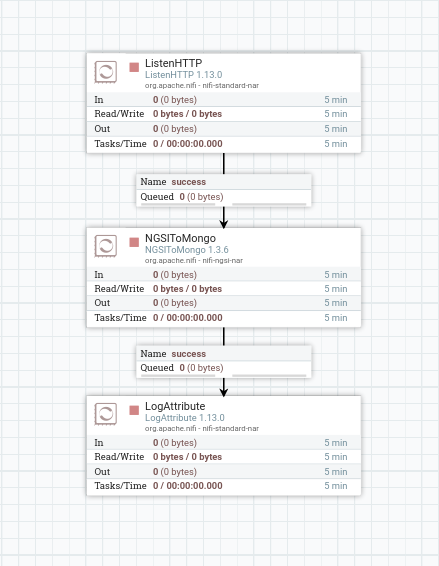
\includegraphics[width=0.7\linewidth]{imagenes/draco-data-routing.png}
	\caption{Graph on Draco UI defining our data routing template}
	\label{draco-data-routing}
\end{figure}

The next step to finish the configuration of Draco will be to edit the parameters of the NGSIToMongo module, so it can properly connect to our database. There, we will configure values like our Replicaset URI, authentication, and the name of the collection.

Once this is done, we can start the Pipeline and Draco will start receiving notifications from Orion once new predicted values arrive. In the following chart, we can see the previous flow updated to include Draco.

\begin{figure}[H]
	\centering
	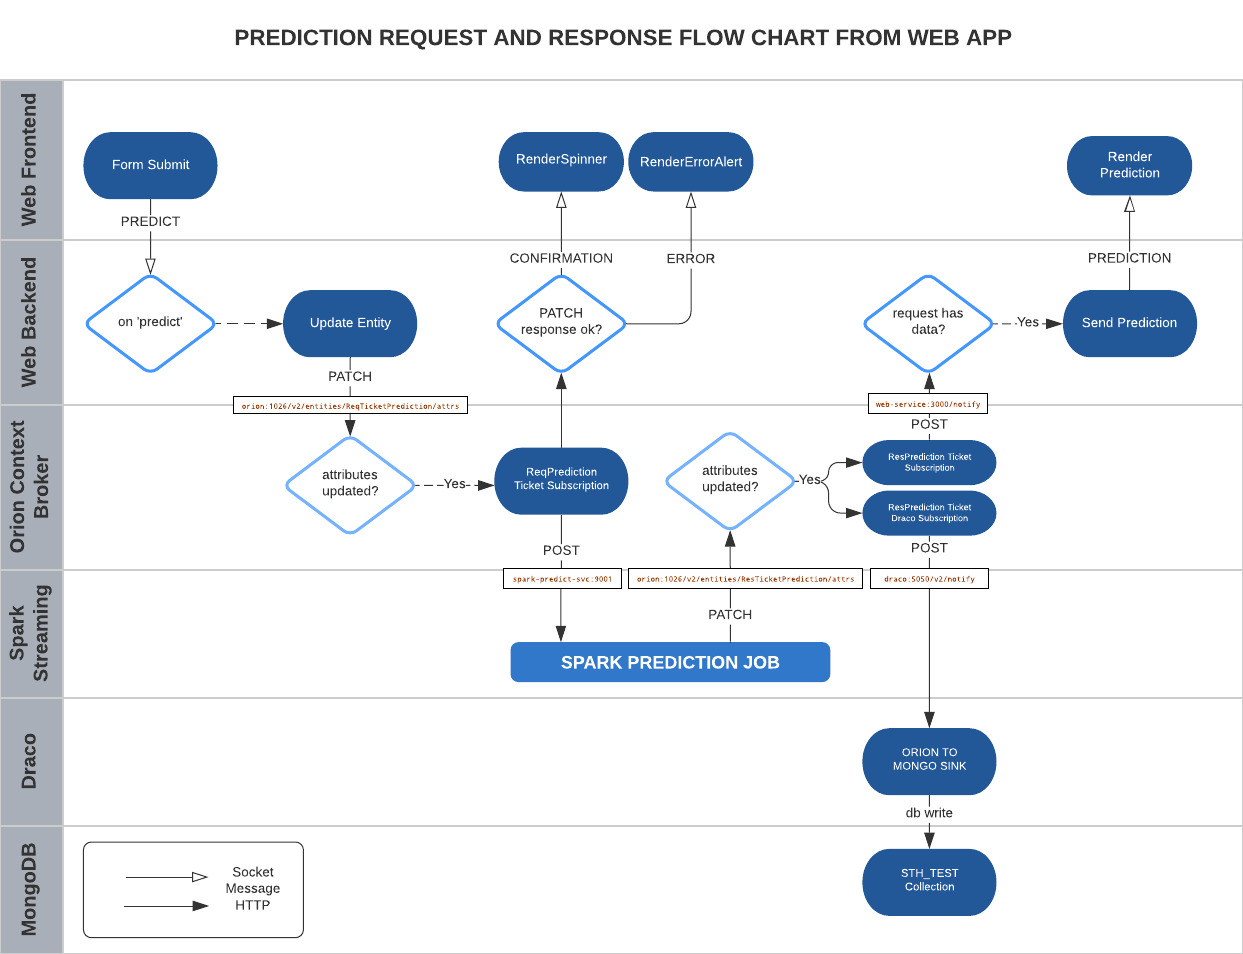
\includegraphics[width=1\linewidth]{imagenes/flow-chart-web-draco.png}
	\caption{Prediction request and response flow chart from webapp to draco.}
	\label{flow-chart-web-draco}
\end{figure}

\clearpage

\section{Machine Learning Model}
\label{section:ML}

In this section, we will discuss the data collection, analysis, and processing stages, as well as the model selection and training, both in Python and in Scala. 

As we discussed in the introduction of this chapter, the data is exposed by a public entity that belongs to the Málaga town hall, SMASSA \cite{smassa}. They are in charge of managing and solving the problems of the public parking of the city, and they are linked to the city Open Data portal, where public data from different sources is exposed so everybody can work with them and collaborate in creating a better and smarter city.

In the Open Data Portal of the Málaga town hall\cite{OpenDataParkingMalaga} , we can find an endpoint where data regarding the parking available spots is published, and this will be our main data source. Unfortunately, they do not have available yet a dataset with past data, and they only publish a new JSON or CSV document every minute with the real-time values for all the Parkings of the city, so we had to come up with a solution to have a dataset to train our model. 

We will go in deep on this solution in the next section, so for now let's suppose that all the data is already in our MongoDB database as raw data in the NGSIv2 JSON format.

\subsection{Our source data}

Our system has collected data since it started working, on July 27th of 2021, and besides some corrupted data on a couple of weeks in September, it has been working until the end of the year. This may seem as not enough data to feed a sufficiently good machine learning algorithm, but the results so far are acceptable, and the idea is that if we maintain this system running in the future, it will automatically fetch new data each minute, and train the model every month adding the new information to the dataset, so the model will improve over time. 

There is available data for ten public parking facilities around the city, and as the data is gathered every minute, we have almost 3.000.000 values in total on the day this document is written. The availability data is exposed in the FIWARE NGSI format, where a lot of context information about the location and facility where the value was produced is added, with the idea of allowing different types of integrations. Here, you can see an example of a value fetched from the portal: 

\begin{lstlisting}[language=json, caption=Example of a NGSI JSON object fetched from the Málaga Town Hall Open Data Portal.]
{ 
    "name": {
        "type": "Text", 
        "value": "Salitre"
    }, 
    "availableSpotNumber": {
        "type": "Integer", 
        "value": "168", 
        "metadata": {
            "timestamp": {
                "type": "DateTime", 
                "value": "None"
            }
        }
    }, 
    "source": {
        "type": "Text", 
        "value": "https://datosabiertos.malaga.eu/recursos/aparcamientos/ocupappublicosmun/ocupappublicosmunfiware.json"
    }, 
    "totalSpotNumber": {
        "type": "Integer", 
        "value": -1
    }, 
    "location": {
        "type": "geo:json", 
        "value": {
            "type": "Point", 
            "coordinates": ["-4.4276681", "36.7132149"]
        }
    },  
    "owner": {
        "type": "Text", 
        "value": "https://www.smassa.eu/"
    }, 
    "occupancyDetectionType": {
        "type": "Array", 
        "value": ["singleSpaceDetection"]
    }, 
    "dataProvider": {
        "type": "Text", 
        "value": "https://www.smassa.eu"
    }, 
    "type": "OffStreetParking", 
    "id": "Salitre", 
    "description": {
        "type": "Text", 
        "value": "Calle SalitreM\u00e1laga"
    }
}
\end{lstlisting}

Some of the values have been suppressed, as they were not relevant for our example. Here, we can see the Parking name and the number of available spots at that time, along with other values as the location of the facility, the type of parking, or the type of detection used for doing the calculation. 

All the data is described using an Open Data format, where each value has a type field describing the Context of the value. As you can see, the Date and time information is not included in the provided data, but we have solved this by editing the DateTime value in the metadata field at the time of the data harvesting. We will describe this modification in the next section. The data regarding the total number of available spots for parking in each facility was also missing, but we found this data in the SMASSA webpage, and we have created an object to use these values in the data transformation stage. 

The interesting values for us are the Parking ID, the date and time the value was generated, and the available spot number for this combination. Starting from here, we deployed a Jupyter notebook in our Kubernetes cluster to analyze and test the data. This makes it easier to understand how are the values distributed across time, and test which machine learning classification model fits better our needs. 

\clearpage

\subsection{Data transformation and analysis}

For the data analysis and inspection, we loaded all the values from October and November to the notebook, using the \textit{pymongo}\cite{pymongo} library to connect to the database service and fetch the documents. We only want to keep some of the values that actually form the object, so we will create a new pandas DataFrame with these values, and start the data processing. The steps we followed to prepare and transform the data, as a brief summary are:

\begin{itemize}
    \item Extract the data from the raw JSON object and create a new dataframe, containing the Parking ID, the DateTime string, and the number of available spots.
    \item Transform the Parking name so it doesn’t include any exceptional character that could be wrongly processed by the algorithm, as accents or whitespaces.
    \item Convert the date and time string to a proper DateTime object, which will be converted to date and time-related values in the following steps.
    \item Convert the number of available spots in an Integer, and drop the not available values from the DataFrame. Not available values are defined as a -1 if they were generated by the source, and a None value if they were corrupt or wrongly processed at the fetching time. We should handle both cases.
    \item We will add the total number of spots for each facility from a statically-generated list.
    \item We will calculate the occupation of the facility for each value dividing the available spots by the total number of spots in the facility, and then rounding it and inverting the value. This will result in a percentage of the occupation, in intervals of 10%.
    \item From the datetime object, we will extract interesting data for our model, as the day of the week, the day, the hour, or the month when the value was generated.
\end{itemize}

After this first pre-processing, we inspected the data to search for patterns and interesting correlations between input data. This is the head of our DataFrame at this point of the analysis (Figure \ref{dataframe-no-preprocessing}):

\begin{figure}[H]
	\centering
	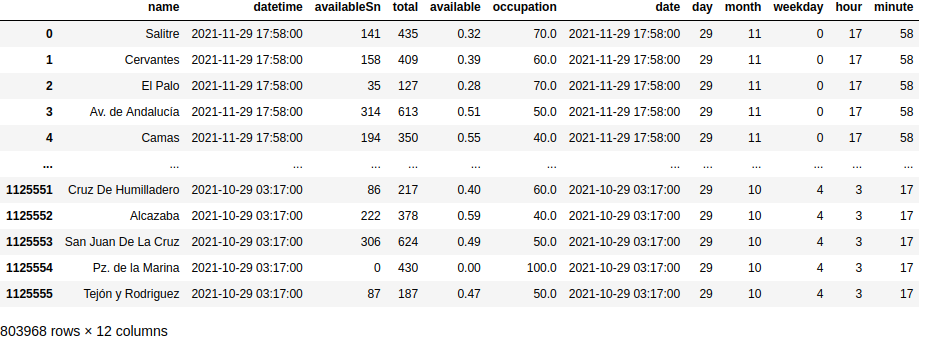
\includegraphics[width=1\linewidth]{imagenes/dataframe-no-processing.png}
	\caption{Dataframe after data preprocessing. Some interesting insights were extracted from the original values.}
	\label{dataframe-no-preprocessing}
\end{figure}

Now we can represent this data to search patterns. First, we represented the occupation level for each parking facility in intervals of 4 hours, and we can plot it as a line plot (Figure \ref{parking-occupation-time}). This is not the cleanest way of visualizing the data, but it can help to visualize the occupation of each parking independently through time.

\begin{figure}[H]
	\centering
	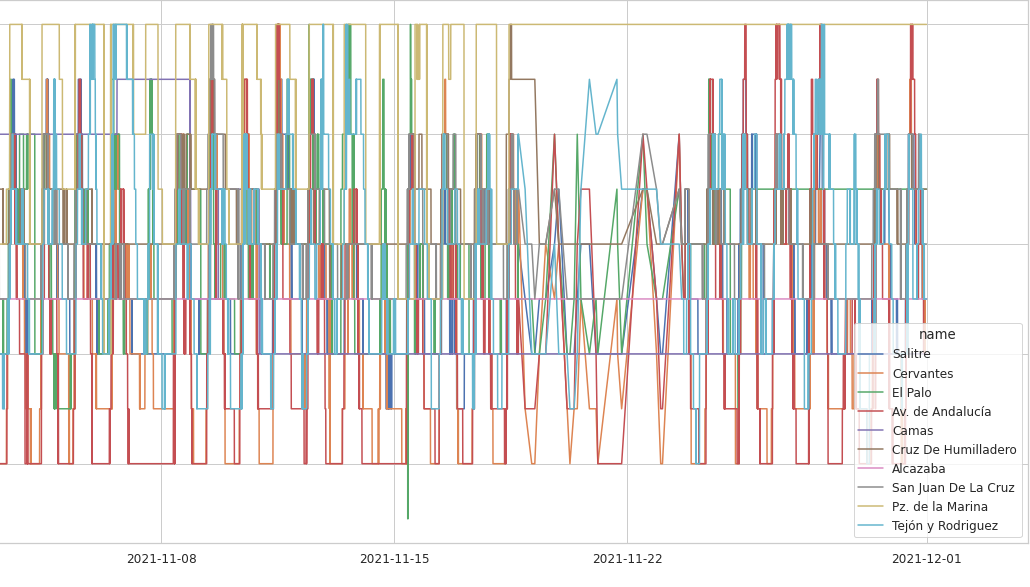
\includegraphics[width=1\linewidth]{imagenes/parking-occupation-time.png}
	\caption{Parkings occupation through time (October and November).}
	\label{parking-occupation-time}
\end{figure}

For a cleaner visualization, we can do the same but aggregating the values by the mean of all the facilities for a certain time interval (Figure \ref{parking-mean-occupation-time}). Here, we can start to see some patterns, depending on the time of the day and the day of the week. We can easily detect the bigger affluence on the weekends, as well as the increase of the occupation in the holidays.

\begin{figure}[H]
	\centering
	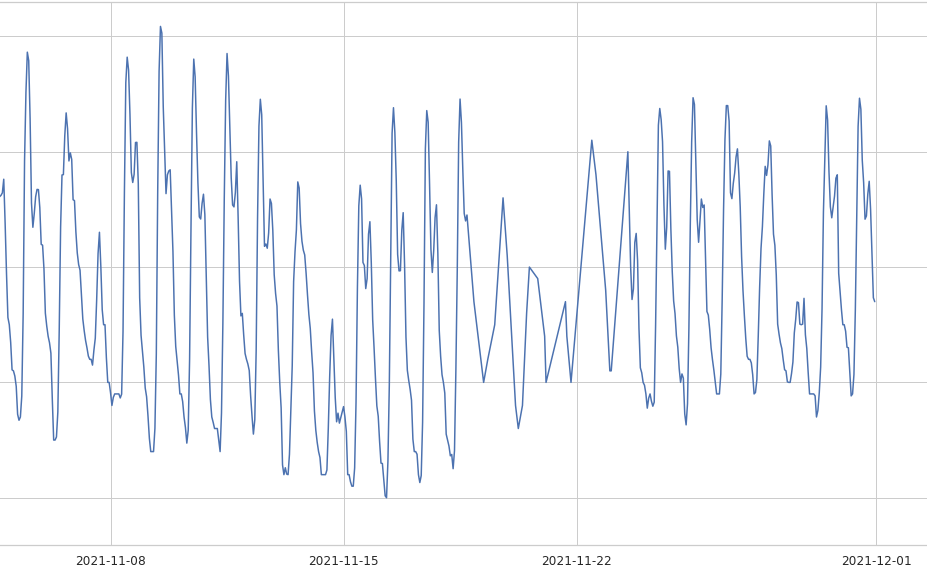
\includegraphics[width=1\linewidth]{imagenes/parking-mean-occupation-time.png}
	\caption{Parkings occupation through time (October and November).}
	\label{parking-mean-occupation-time}
\end{figure}

Focusing on these patterns, we can further explore them by aggregating the data for each feature. We can, for example, plot the mean occupancy for each day of the week, or by the time of the day. This way, we obtain these really interesting graphs.

In this first plot, we can see how the day of the week is somehow important for the occupation level, but it depends on the parking facility. Also, we can extract that depending on the parking, the occupation will increase on the weekends, or decrease, probably based on its location. Parking lots close to work areas outside of the city center will have lower affluence on the weekends, while those in the city center will tend to be more crowded.

\begin{figure}[H]
	\centering
	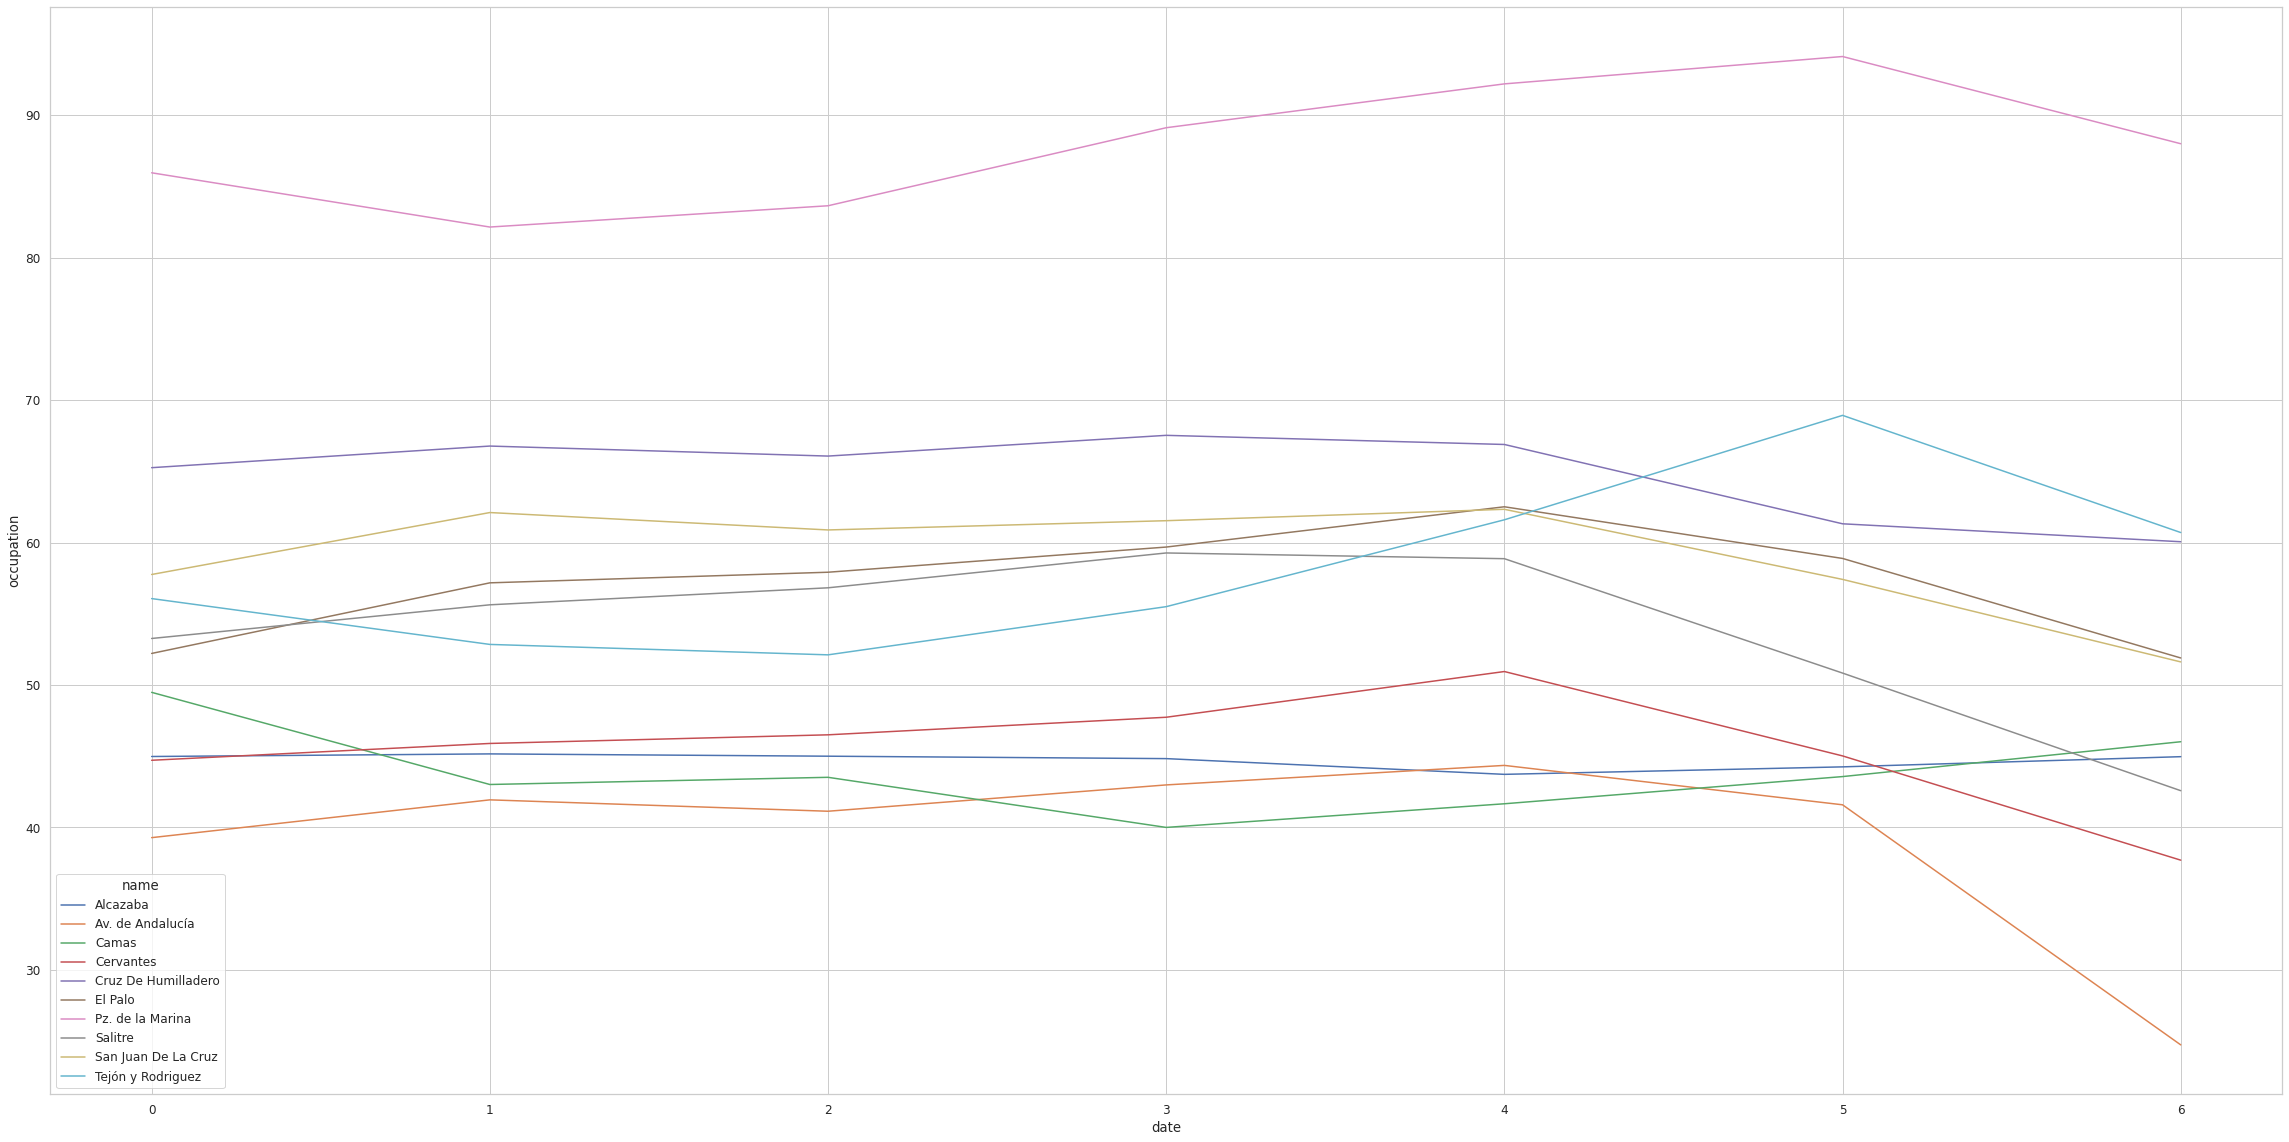
\includegraphics[width=0.9\linewidth]{imagenes/aggregated-mean-occupation-week.png}
	\caption{Aggregated mean parking occupation depending on the day of the week (0-Monday, 6-Sunday).}
	\label{aggregated-mean-occupation-week}
\end{figure}

On the other hand, if we look at the aggregated occupation depending on the hour of the day, we could see a strong correlation for most of them, decreasing the occupation during the night and with a strong increase in the morning.

\begin{figure}[H]
	\centering
	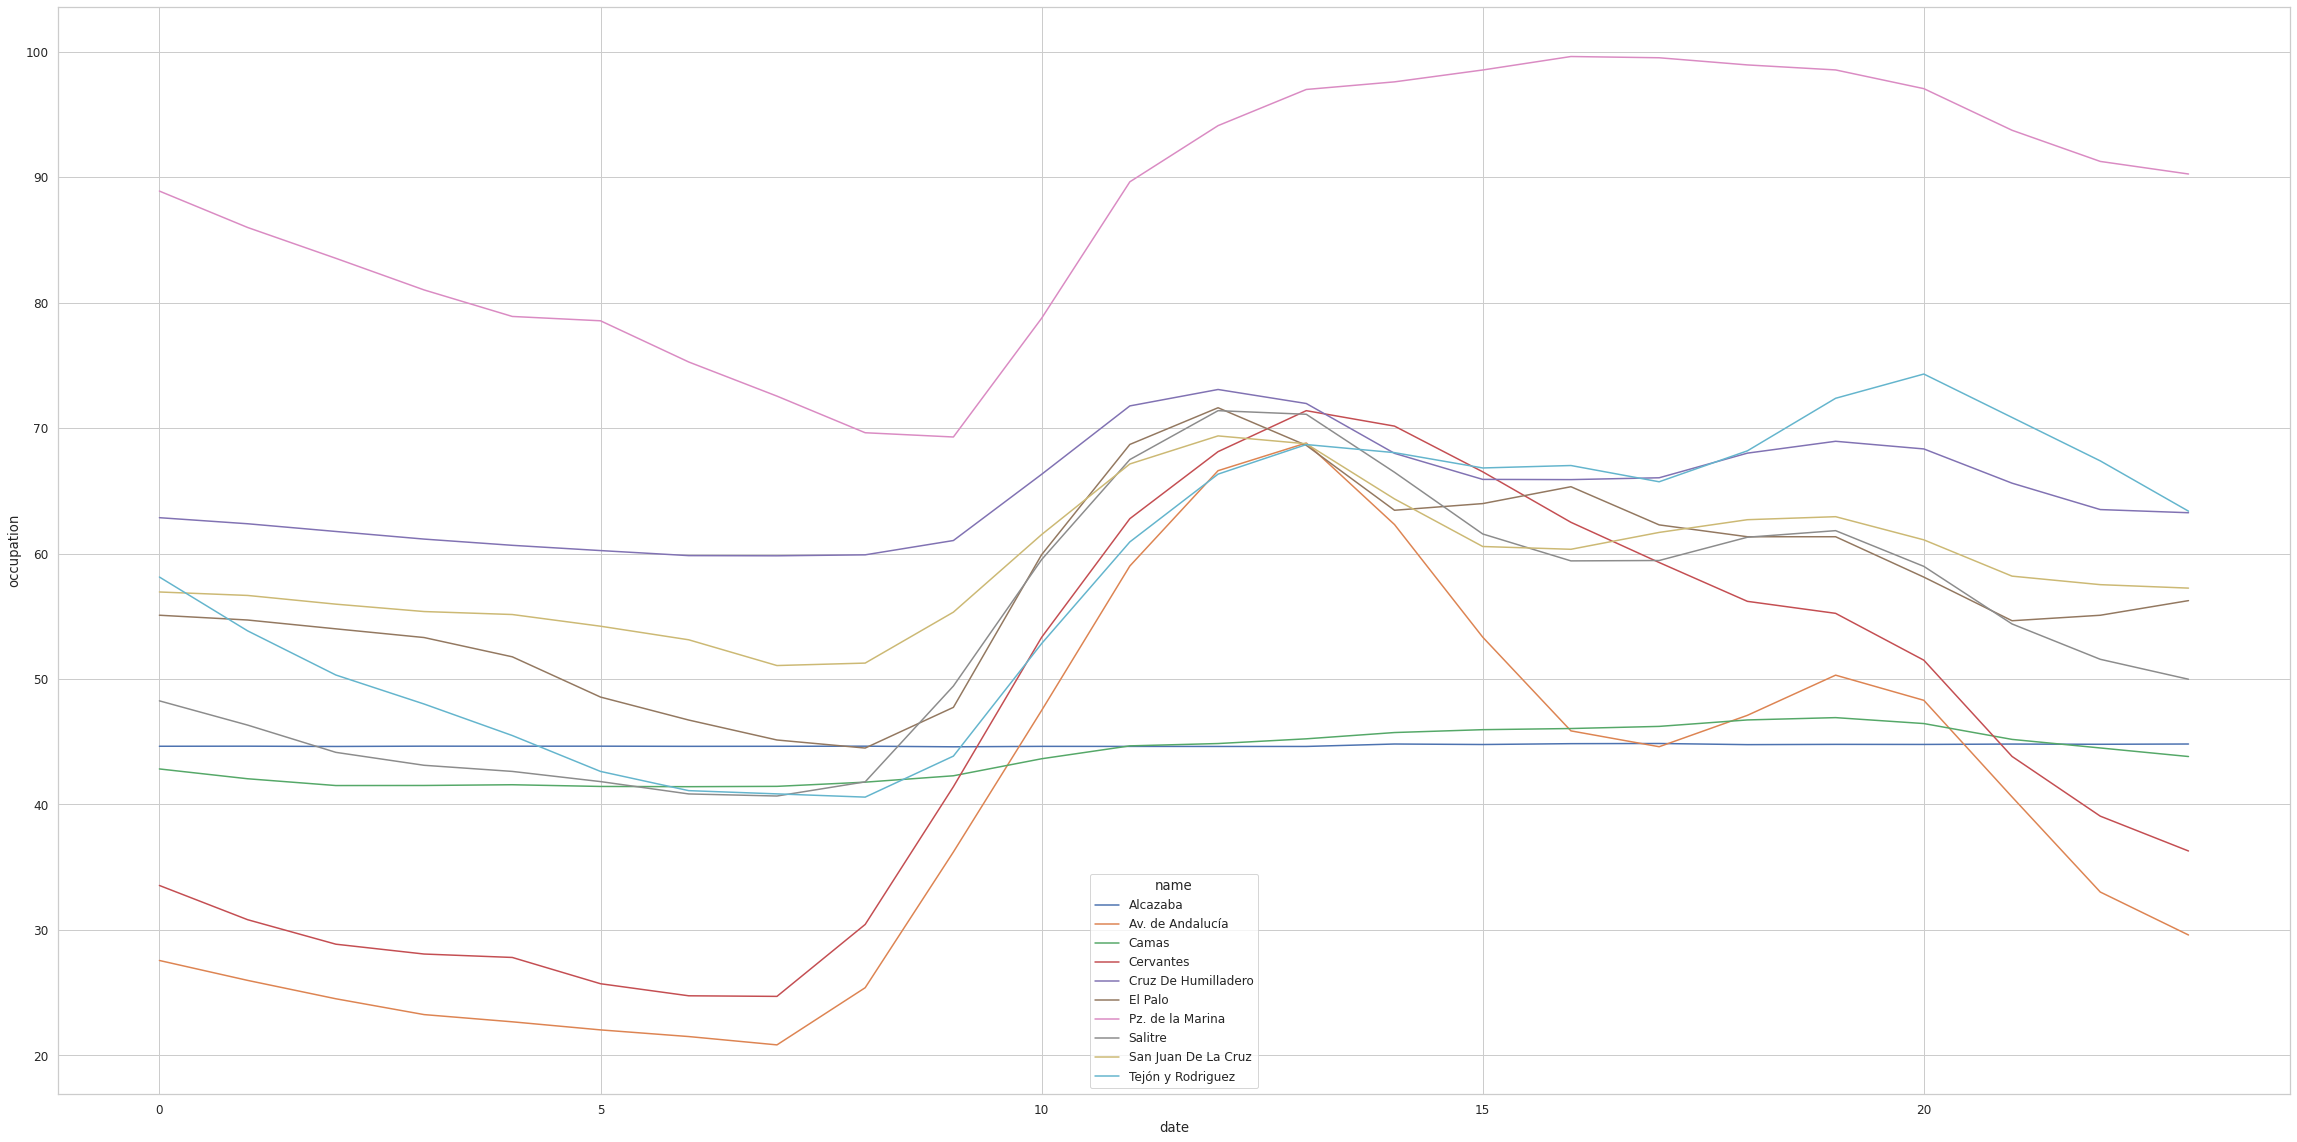
\includegraphics[width=0.9\linewidth]{imagenes/aggregated-mean-occupation-hour.png}
	\caption{Aggregated mean parking occupation depending on the hour of the day.}
	\label{aggregated-mean-occupation-hour}
\end{figure}

Also in this graph, we noticed that the values for the facilities of Alcazaba and Camas are almost continuous, and after a deeper look into the data, we found that the values for Alcazaba were odd, having its occupation around 45 percent for the whole period when data was been collected. This forced us to discard this facility for the moment, until we have better data.

\clearpage

\subsection{Model selection}

After processing the data, our next step is to select the best features and compare training results on different models. We did this on our Jupyter Notebook, and in the following sections we will move our model to Scala in order to integrate it with our system.

Due to the lack of data from previous years, it doesn't seem like the feature year will have any weight in the predictions, so we discarded it for now. Taking this into account, we have five features to work with: The facility name, which we will index in order to pass it to the model, and the time variables like the hour, day, weekday (also indexed from 0-Monday to 6-Sunday), and the month. These are the different available features.

\begin{table}[H]
    \begin{tabular}{|c|c|c|c|c|c|c|}
    \hline
    \textbf{Feature} & name            & hour         & weekday      & day          & month        & \begin{tabular}[c]{@{}c@{}}occupation\\ (label)\end{tabular} \\ \hline
    \textbf{Type}   & \textit{String} & \textit{Int} & \textit{Int} & \textit{Int} & \textit{Int} & \textit{Int}                                                 \\ \hline
    \textbf{Values}       &  "Name"   & {[}1-24{]}   & {[}0-6{]}    & {[}1-31{]}   & {[}1-12{]}   & {[}0:10:100{]}\%                                             \\ \hline
    \end{tabular}
    \caption{Features name, type and available values.}
\end{table}

There are two different approaches on how to face our model search, as we first have to decide if we can face this problem as a classification or a regression problem. Our variable to predict is given as a continuous value, as the available number of spots in each parking facility for a given time. We could feed this data to a regression model, and try to predict the available number of parking spots comparing it to the existing values and extracting, for example, the RMSE (rooted mean square error) to evaluate the model. The other option is to manipulate the label variable so we can convert our label into a categorical variable, as the percentage of occupation from 0 to 100 percent, in intervals of 10 units. This second approach will simplify the complexity of our model, and increase its accuracy. As we don’t need the exact value of available spots, an estimation of the occupation of the facility seems like an easier and more precise model, so we will proceed with this solution.

We will select six classification models, and we will compare all of them setting up a cross-validation function that will provide us a more reliable evaluation of each individual model, so we can have a better overview of which models work better for our data. We will do this process several times, changing the provided set of features so we can compare how different combinations perform.

The models we will tests are:
\begin{itemize}
    \item \textbf{LogR}: Logaritmic Reggresor
    \item \textbf{LDA}: Linear Discrimination Analysis
    \item \textbf{KNN}: K-nearest Neighbors
    \item \textbf{DTC}: Decision Tree Classifier
    \item \textbf{RFC}: Random Forest Classifier
    \item \textbf{SGD}: Stochastic Gradient Descent Classifier
\end{itemize}

And the acronyms used for the feature variations are:
\begin{itemize}
    \item \textbf{NM}: Month feature not included
    \item \textbf{M}: Month feature included
    \item \textbf{NI}: Name feature indexed
    \item \textbf{NC}: Name feature codified
    \item \textbf{WC}: Week feature codified
\end{itemize}

\begin{table}[H]
    \begin{tabular}{|l|l|l|l|l|l|l|}
    \hline
    \textbf{Ft}                                                  & \textbf{LogR}                                        & \textbf{LDA}                                                  & \textbf{KNN}                                                  & \textbf{DCT}                                              & \textbf{RF}                                                   & \textbf{SGD}                                                 \\ \hline
    \textit{\begin{tabular}[c]{@{}l@{}}NI \\ NM\end{tabular}}    & \begin{tabular}[c]{@{}l@{}}0.44423\\ (0.00196)\end{tabular} & \begin{tabular}[c]{@{}l@{}}0.42004\\ (0.001)\end{tabular} & \begin{tabular}[c]{@{}l@{}}0.54821\\ (0.00227)\end{tabular} & \begin{tabular}[c]{@{}l@{}}0.58465\\ (0.00181)\end{tabular} & \begin{tabular}[c]{@{}l@{}}0.58483\\ (0.00192)\end{tabular} & NA                                                           \\ \hline
    \textit{\begin{tabular}[c]{@{}l@{}}NI\\ M\end{tabular}}      & \begin{tabular}[c]{@{}l@{}}0.44423\\ (0.00196)\end{tabular} & \begin{tabular}[c]{@{}l@{}}0.42023\\ (0.00184)\end{tabular} & \begin{tabular}[c]{@{}l@{}}0.54212\\ (0.00204)\end{tabular} & \begin{tabular}[c]{@{}l@{}}0.59463\\ (0.00136)\end{tabular} & \begin{tabular}[c]{@{}l@{}}0.59502\\ (0.00127)\end{tabular} & \begin{tabular}[c]{@{}l@{}}0.38345\\ (0.00593)\end{tabular} \\ \hline
    \textit{\begin{tabular}[c]{@{}l@{}}NC\\ M\end{tabular}}      & \begin{tabular}[c]{@{}l@{}}0.45317\\ (0.00135)\end{tabular}  & \begin{tabular}[c]{@{}l@{}}0.4216\\ (0.00150)\end{tabular}  & \begin{tabular}[c]{@{}l@{}}0.54927\\ (0.00269)\end{tabular} & \begin{tabular}[c]{@{}l@{}}0.59480\\ (0.00129)\end{tabular} & \begin{tabular}[c]{@{}l@{}}0.59451\\ (0.00166)\end{tabular} & \begin{tabular}[c]{@{}l@{}}0.4012\\ (0.00751)\end{tabular} \\ \hline
    \textit{\begin{tabular}[c]{@{}l@{}}NC\\ WC\\ M\end{tabular}} & \begin{tabular}[c]{@{}l@{}}0.42142\\ (0.00169)\end{tabular}  & \begin{tabular}[c]{@{}l@{}}0.41991\\ (0.00168)\end{tabular} & \begin{tabular}[c]{@{}l@{}}0.54811\\ (0.00254)\end{tabular} & \begin{tabular}[c]{@{}l@{}}0.59648\\ (0.00168)\end{tabular} & \begin{tabular}[c]{@{}l@{}}0.61502\\ (0.00100)\end{tabular} & \begin{tabular}[c]{@{}l@{}}0.41531\\ (0.0102)\end{tabular} \\ \hline
    \end{tabular}
    \caption{Comparaison of cross-validation evaluation results for different classification models and feature combination. Mean accuracy and standart deviation.}
\end{table}

These results were obtained through a k-fold Cross-Validation method. Specifically, we used a 10-fold random validation, so for each model, we performed the training process using one of each 10 splits of the dataset as our test data, and the other 9 as the train data, obtaining an array of evaluations, in this case the accuracy. Then, what is displayed is the mean accuracy and the standard deviation for the specific model. \\

\begin{lstlisting}[language=Python, caption=Portion of the code we used for the cross-validation of the models]
for name, model in models:
	kfold = model_selection.KFold(n_splits=10, random_state=seed,shuffle=True)
	cv_results = model_selection.cross_val_score(model, X, Y, cv=kfold, scoring='accuracy')
	results.append(cv_results)
	names.append(name)
	msg = "%s: %f (%f)" % (name, cv_results.mean(), cv_results.std())
\end{lstlisting}

As the algorithm that outperformed the others was the Random Forest Classifier, we tried to improve its results by tuning the hyperparameters. In order to search for the best combination of inputs, we performed a GridSearch, that evaluates the model using cross-validation for different parameters, and outputs the combination of values that showed a better result.

We performed this grid search modifying the number of trees, from 200 up to 700, and by changing the max-features parameter of the algorithm. This defines the maximum number of features Random Forest is allowed to try in an individual tree, and there are three available options. Basically, this limits the number of features allowed up to the number of features provided (auto), up to the square root of the number of features (sqrt) or up to the base two logarithm of the number of features (log2). \\

\begin{lstlisting}[language=Python, caption=Portion of the code we used for performing the parameters grid search.]
rfc = RandomForestClassifier(n_jobs=-1,max_features= 'sqrt' ,n_estimators=50, oob_score = True) 
param_grid = { 'n_estimators': [200, 700],'max_features': ['auto', 'sqrt', 'log2']}
CV_rfc = GridSearchCV(estimator=rfc, param_grid=param_grid, cv= 5)
CV_rfc.fit(X, Y)
print(CV_rfc.best_params_)
\end{lstlisting}

With this tuning, we found that the best parameters for this setup were \textit{'max\_features': 'log2', 'n\_estimators': 200}, and after doing a new cross-validation with these parameters, we managed to increase the accuracy up to 0.662830 (0.001354). Doing a deeper analysis of the final model metrics, we obtained the confusion matrix and confidence intervals before moving to Scala.

\begin{figure}[H]
	\centering
	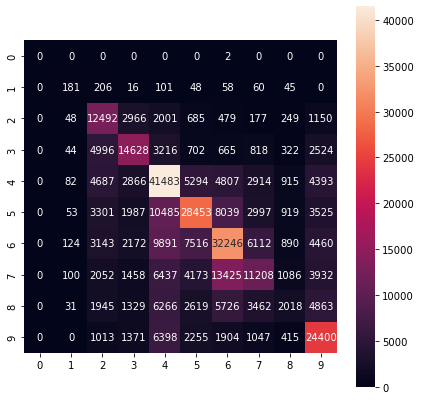
\includegraphics[width=1\linewidth]{imagenes/confusion-matrix.png}
	\caption{Confusion matrix representing our 10 target classes for our final model}
	\label{confusion-matrix}
\end{figure}

As we can see from Figure \ref{confusion-matrix}, even when our accuracy is not really good, the predictions are usually close to the target category, and we have to take into account the fact that our dataset is still limited. This issue should be solved in the future as the dataset grows bigger and consequently, our model has more inputs to learn the problem better.

In the next section, we will move our model to Spark, to deploy it in our Kubernetes cluster and integrate it with our complete workflow.

\clearpage

\section{Spark and Spark Streaming}
\label{section:Spark}
Apache Spark\cite{spark} is an open-source programming framework for distributed data processing designed to be fast and general purpose\cite{spark}. It can quickly perform processing tasks on very large data sets, and can also distribute data processing tasks across multiple computers. These properties fit really good our project needs, so it can be a perfect solution for our data processing stage.

Spark is designed for running Big Data and Machine Learning tasks at scale, as it has been designed from the core to be able to parallelize and break up tasks in smaller pieces, that we can distribute in multiple servers for processing them, and that later can be combined again to get I final result. In our system, we will use Spark for training our models, and later, use those models to make predictions on incoming requests, using Spark Streaming.

We have two options for deploying a Spark application to a cluster, \textbf{Client mode}, and \textbf{Cluster mode}. The main difference is where will the driver application run, and depending on your system requirements and where are you deploying this app, one option will be better than the other. In our case, as our development environment is separated from our cluster, we will opt for the Cluster mode approach.

\begin{figure}[H]
	\centering
	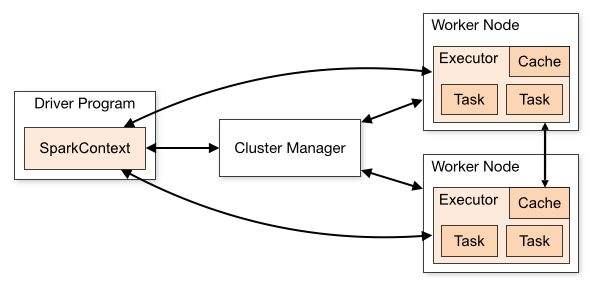
\includegraphics[width=1\linewidth]{imagenes/spark-modes.png}
	\caption{Spark application architecture. From Apache Documentation\cite{spark}.}
	\label{spark-modes}
\end{figure}

As we are deploying our Spark applications to Kubernetes, we have two options depending on our system specifications. Spark adopts a Master/Slave approach whereby a \textit{driver program} (“the master”) creates a \textit{SparkContext} object that connects to a \textit{cluster manager}. This SparkContext is actually an abstraction of the system where it will be executed, and uses it as a unique node where tasks are distributed. The difference then lies in where the cluster manager runs, and even though Kubernetes is supported as a cluster manager since the last Spark update, we stuck to the Standalone cluster manager, where it will run in the node we use for development (outside of the cluster), and will behave as a fire-and-forget process.

Once we submit our Spark application using the spark-submit tool shipped with the spark binaries, it will create a SparkContext (defined in the application code), that will ask the kube-apiserver to set up a driver Pod using a specific image and deploy some executors. Then it will proceed to run the workload on them.

\subsection{Model definition in Spark. Train and Prediction jobs}

In the first iterations of the project, we developed everything with PySpark and MLib, two frameworks for developing Spark applications for machine learning with Python, as we had the advantage of being able to use Jupyter notebooks shipped with Spark to test and debug the code. But after some iterations, we found a lot of issues with the dependencies, and some versions were incompatible with the rest of our Cluster. Also, the Orion connector for Spark was already developed for Scala, and after some failed attempts to adapt it to PySpark, we decided to move all our code to Scala.  

The project will be built using Scala version \textit{2.12.13} and Spark \textit{3.0.1}, so we can be compatible with the MongoDB and the Orion connector libraries. We will use SBT \cite{sbt} as our compiler and build tool, so it has to be properly configured with our build and dependencies requirements. First step is to define our \textit{build.sbt} configuration file to include the required dependencies and our build versions. The idea is to create a fat jar binary that will be shipped with the Docker image to the cluster, and the instructions on how to run the programs will be defined in the SparkContext.

The required additional dependencies that we must include are:
\begin{itemize}
    \item \textbf{Spark MLlibs:} The library for creating and executing machine learning models on Spark\cite{ml-spark}.
    \item \textbf{MongoDB Spark Connector:} With the connector, we will have access to all Spark libraries for use with MongoDB datasets. We will use this connector to fetch the training data from the Parking collection.
    \item \textbf{Orion Spark Connector:} Used for interacting with the Orion NGSI API, receive notifications and send a reply with the results.
\end{itemize}

We will define two main Scala classes, Train and Pedict. The \textbf{Train} object, will trigger a SparkSession that will be in charge of:
\begin{itemize}
    \item Start the Spark Session and pass the Context to the executors.
    \item Connect to the MongoDB and fetch the whole parking dataset.
    \item Convert the raw data from the received RDD to a Dataframe.
    \item Transform the data to obtain the desired features and index and encode the required ones.
    \item Define the RandomForestClassifier model with the expected parameters.
    \item Train the whole Pipeline and the model with the DataFrame.
    \item Evaluate the model and store the results for future comparaison.
    \item Save the model and the processing pipeline in the cluster storage.
    \item End the session.
\end{itemize}

The \textbf{Predict} class, on the other hand, will create a Spark Streaming Session instead of the standart one. As we already explained in the previous chapter \ref{chapter:StateOfArt}, Spark Streaming extends Spark focusing on live data streams processing, providing us with better tools to keep our system listening for new prediction on real time. Predict object, will handle the following tasks:

\begin{itemize}
    \item Start the Spark Streaming Session, and pass the Context to the executors.
    \item Start event streams listen service for notifications on the port 9001.
    \item Receive the prediction notification from Orion, and create a Streaming RDD with the request payload.
    \item Load the model and the processing pipelines from the cluster storage.
    \item Transform the request data using the Pipeline, and select the required features.
    \item Generate a prediction of the occupation using the trained model.
    \item Generate a response with the prediction, and send it back to Orion using the Orion Connector.
    \item Keep listening for new prediction streams.
\end{itemize}

We will compile both classes using the sbt assembly command, generating a jar file including all the required dependencies and classes, ready to ship. 

The last step is to generate a Docker image suitable for both our driver node and the executors, and for that we will use the Dockerfile provided with the Spark source. After the image with our sources is created, the last step is to submit our Spark Jobs to the Kubernetes cluster.

\subsection{Model deployment to Kubernetes}

For submitting our Jobs to Kubernetes in Cluster mode\cite{kubernetes-spark}, we will use the tool spark-submit, provided with the Spark sources. This command line tool accepts multiple parameters for configuring all the Spark environment, and it can connect to a Kubernetes Cluster and create all the resources for us if we specify so.

From the same command, we will trigger the creation of the Spark Cluster in Kubernetes, using the Docker image previously generated as the base image for both our driver program and the required executors. We will go through some of the main parameters we used for submitting our job:

\begin{itemize}
    \item \textit{\textbf{master} k8s:CLUSTER-IP:8443}
    \item \textit{\textbf{deploy-mode} cluster}
    \item \textit{\textbf{class} org.fiware.cosmos.orion.spark.connector.prediction.Train}
    \item \textit{\textbf{conf} "spark.executor.instances=1", "cores=4", "memory=12G"}
    \item \textit{\textbf{conf} "spark.kubernetes.driver.label.job=train"}
    \item \textit{\textbf{conf} "spark.kubernetes.persistentVolumeClaim.claimName=spark-pvc"}
    \item \textit{\textbf{conf} "spark.kubernetes.persistentVolumeClaim.path=./models/" }
    \item \textit{\textbf{jar} "spark/jars/tfm-assembly.jar"}
\end{itemize}

These are the main parameters we need to configure our Spark cluster on Kubernetes. Here, we are specifying first the IP of our Kubernetes (in this case Minikube) cluster, and the deploy mode. Then, we have some configurations related to the resources provided to the Pods, in this case we will set up 2 executors with 4 processing cores each and 12Gb of memory for the Training process. We also need to specify the Scala class to use along with the path of the jar file containing our compiled jobs, and finally connect the Pod with the Volume resource where we will store the final models.

We also deployed some additional Kubernetes resources to connect our Spark cluster with the rest of the services, specifically, we created a Service to expose the prediction driver Pod, on port 9001, so the Job can receive notifications from Orion, and also a service to expose the Spark's driver UI, on port 4040. Additionally, we will create a PersistentVolume object that will persist the saved models in the cluster storage, and also share the directories between Train and Prediction jobs.

The final architecture of the Spark cluster on Kubernetes will be as represented in Figure \ref{diagram-spark-kube}.
\begin{figure}[H]
	\centering
	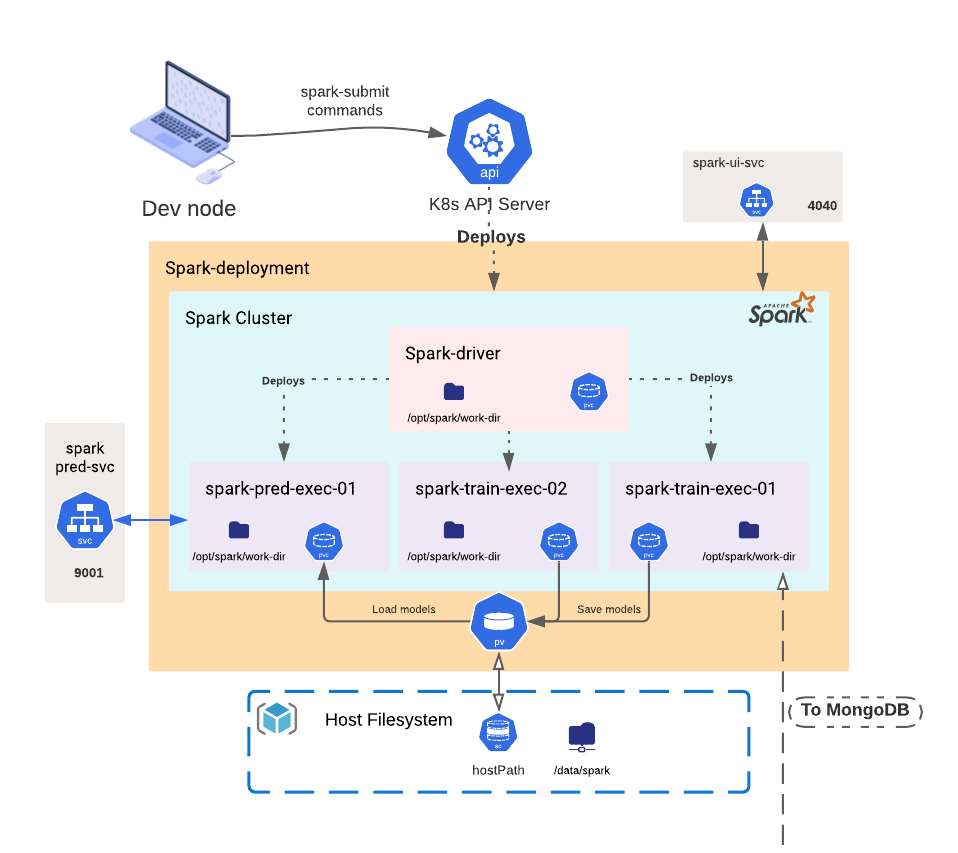
\includegraphics[width=0.9\linewidth]{imagenes/diagram-spark-kube.png}
	\caption{Spark on Kubernetes deployment architecture.}
	\label{diagram-spark-kube}
\end{figure}

\clearpage

\section{Additional Jobs and Modules}

In order to complete the Kubernetes deployment of the whole system, we created some additional items to automate some tasks and improve the reliability of the system over time. 

As we already mentioned in previous sections, we deployed a \textbf{Jupyter Notebook} environment for doing the data analysis and model comparison.

\begin{figure}[H]
	\centering
	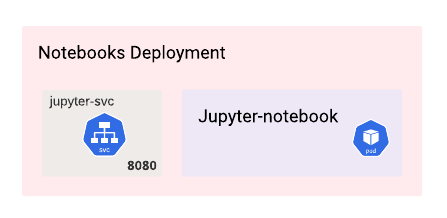
\includegraphics[width=0.6\linewidth]{imagenes/diagram-jupyter.png}
	\caption{Deployment and service architecure for the notebooks environment.}
	\label{diagram-jupyter}
\end{figure}

Additionally, we created two more resources to help us automate some tasks. Both items are what Kubernetes defines as Jobs or CronJobs, and are basically Pods that are deployed under certain conditions to complete a task, and then they are deleted.

The first Job will be a \textbf{data sink}. As the data we are using is exposed for one minute and then overriden by the new value in the Málaga Town Hall Open Data Portal, we need a way to keep a register of past values for training our model. 

We developed a Python script that scrapes the website and saves the data to our MongoDB database as a raw JSON. With the help of the Kubernetes CronJob resource and this script, we can save all the information in our database for future access, running the script every minute and logging the time of the download in the document metadata. 

For doing this, we created a light Docker image with the script loaded, and created the resource in Kubernetes so it runs every minute while the cluster is up. This is the way we acquired all the data used to train the model since the beginning of the development.

\begin{lstlisting}[language=yaml,caption=Kubernetes YAML definition file for the sink CronJob]
apiVersion: batch/v1
kind: CronJob
metadata:
  name: sink-job
  namespace: tfm
spec:
  schedule: "*/1 * * * *"
  jobTemplate:
    spec:
      template:
        spec:
          containers:
          - name: sink-job
            image: tonihurtado/sinkjob:latest
            imagePullPolicy: IfNotPresent
            command: ["python3", "/app/update-db.py"]
          restartPolicy: OnFailure
\end{lstlisting}
\label{section:Add}

The other CronJob, will have the task of running our training Job every month, with the new data scraped with the Sink Job. It will run on the first day of the month, and save the evaluation results on the storage so we can compare the performance of each model.

